% DDS-Edge: nhận diện tài xế mất tập trung trên thiết bị edge (10 lớp)
% Biên dịch: Overleaf, compiler pdfLaTeX. Tải cả thư mục paper/ (gồm figs/).
\documentclass[10pt,a4paper,twocolumn]{article}

\usepackage[T5]{fontenc}
\usepackage[utf8]{inputenc}
\usepackage[vietnamese]{babel}
\usepackage[margin=1.8cm,columnsep=0.6cm]{geometry}
\usepackage{amsmath,amssymb}
\usepackage{graphicx}
\usepackage{booktabs}
\usepackage{multirow}
\usepackage{xcolor}
\usepackage{caption}
\usepackage{enumitem}
\usepackage{pgfplots}
\pgfplotsset{compat=1.17}
\usepackage[hidelinks]{hyperref}

\captionsetup{font=small,labelfont=bf}
\setlist{nosep,leftmargin=*}
\newcommand{\cls}[1]{\texttt{#1}}
\definecolor{dblue}{HTML}{3B6FF0}
\definecolor{dgray}{HTML}{9AA3B2}
\definecolor{dviolet}{HTML}{8E5CF0}
\pgfplotsset{every axis/.append style={/pgf/number format/use comma,
  tick label style={font=\scriptsize}, label style={font=\footnotesize},
  legend style={font=\scriptsize}}}

\title{\textbf{Nhận diện tài xế mất tập trung trên thiết bị Edge:\\
đánh đổi giữa độ chính xác, kích thước và tốc độ}}
\author{Trần Gia Huy\\[2pt]
\small Bài tập lớn môn Deep Learning, dự án DDS-Edge}
\date{}

\begin{document}
\maketitle

\begin{center}
\fbox{\begin{minipage}{0.95\linewidth}\small
\textbf{Tuyên bố sử dụng AI}\\[3pt]
\begin{tabular}{@{}p{0.72\linewidth}l@{}}
1. Sử dụng AI hỗ trợ viết báo cáo & \textbf{Yes} \\
2. Sử dụng AI hỗ trợ sinh các biểu đồ & \textbf{Yes} \\
3. Sử dụng AI sinh giao diện (demo) & \textbf{Yes} \\
4. Sử dụng AI sinh test cases & \textbf{Yes} \\
5. Tỉ lệ sử dụng AI & \textbf{khoảng 70\%} \\
\end{tabular}\\[3pt]
{\footnotesize Công cụ: Claude (Anthropic). AI hỗ trợ viết mã, tài liệu, báo cáo, biểu đồ và test; tác giả đặt câu hỏi nghiên cứu, quyết định thiết kế thí nghiệm, tự chạy huấn luyện trên Colab và kiểm tra kết quả.}
\end{minipage}}
\end{center}

\begin{abstract}
Nhận diện hành vi mất tập trung của tài xế từ camera trong xe cần chạy ngay trên thiết bị đặt trong xe (edge), nơi bộ nhớ, năng lực tính toán và điện năng đều hạn chế. Bài này so sánh bốn mạng tích chập (MobileNetV3-Small, EfficientNet-Lite0, ResNet18, ResNet50) trên bộ State Farm Distracted Driver với 10 lớp hành vi, chia dữ liệu theo tài xế và loại bỏ ảnh gần trùng. Ngoài độ chính xác (macro-F1 trên tài xế chưa từng thấy), chúng tôi đo số tham số, MACs, kích thước, độ trễ và FPS trên CPU, trước và sau lượng tử hoá INT8 sau huấn luyện. Cả bốn mô hình đạt macro-F1 từ 0,83 đến 0,86 trên một lần chia, nhưng cross-validation theo tài xế 5 fold đảo thứ hạng: EfficientNet-Lite0 $0{,}863 \pm 0{,}032$ và ResNet18 $0{,}855 \pm 0{,}039$ không phân biệt được, còn MobileNetV3-Small chỉ $0{,}793 \pm 0{,}057$. Mô hình nặng không chính xác hơn mô hình vừa. Khác biệt lớn nằm ở lượng tử hoá: EfficientNet-Lite0, ResNet18 và ResNet50 giữ nguyên độ chính xác sau INT8 (mất không quá 0,008), nhỏ hơn 3,5 đến 4 lần và nhanh hơn 1,6 đến 3,1 lần, còn MobileNetV3-Small, vốn đã kém hơn ở FP32, sụp từ 0,864 (một lần chia) xuống 0,067. Phân tích riêng từng loại phép toán cho thấy trọng số lượng tử hoá được, còn lượng tử hoá activation của các lớp tích chập mới là nguyên nhân. Lớp yếu nhất là \cls{c9} (nói chuyện với hành khách), chủ yếu bị nhầm với \cls{c8} (chải tóc/trang điểm).
\end{abstract}

\noindent\textbf{Từ khoá:} edge AI, phân loại ảnh, tài xế mất tập trung, lượng tử hoá INT8, mạng nhẹ.

% =====================================================================
\section{Giới thiệu}
Mất tập trung khi lái xe (dùng điện thoại, ăn uống, quay sang hành khách\ldots) là hành vi cần được phát hiện và cảnh báo kịp thời. Một camera trong xe kết hợp với mô hình phân loại ảnh có thể làm việc này. Có hai cách triển khai: gửi ảnh lên máy chủ để suy luận (cloud AI) hoặc chạy mô hình ngay trên thiết bị trong xe (edge AI). Edge AI phù hợp vì cảnh báo không phải chờ đường truyền, video có mặt tài xế không phải gửi đi, và hệ thống vẫn chạy khi xe mất sóng. Cái giá phải trả là thiết bị edge có bộ nhớ, năng lực tính toán và điện năng hạn chế, nên mô hình phải nhỏ và nhanh.

Việc thu nhỏ mô hình để chạy trên edge (chọn kiến trúc nhẹ, lượng tử hoá số thực 32 bit thành số nguyên 8 bit) có thể làm giảm độ chính xác. Câu hỏi nghiên cứu của bài là:
\emph{khi bị giới hạn tài nguyên như thiết bị edge, ta đánh đổi bao nhiêu độ chính xác trên tài xế chưa từng thấy, có cách nào thu hẹp khoảng cách đó, và mô hình nào thực sự khả thi để đưa lên edge?}

Đóng góp của bài:
\begin{itemize}
\item Một giao thức đánh giá cố định trên State Farm: chia theo tài xế để tránh rò rỉ dữ liệu, loại bỏ ảnh gần trùng, dùng macro-F1 trên 10 lớp gốc, và cross-validation theo tài xế để đo độ nhiễu của chính phép đánh giá.
\item So sánh bốn kiến trúc từ 1,5 đến 23,5 triệu tham số về độ chính xác, MACs, kích thước, độ trễ và FPS, trước và sau lượng tử hoá INT8.
\item Chỉ ra rằng khả năng chịu lượng tử hoá, chứ không phải số tham số, quyết định mô hình nào khả thi trên edge, kèm một chẩn đoán từng bước nguyên nhân MobileNetV3-Small không chịu được INT8 sau huấn luyện.
\item Phân tích lỗi theo lớp và theo tài xế, cho thấy giới hạn nằm ở một lớp nhập nhằng (\cls{c9}).
\end{itemize}

% =====================================================================
\section{Công trình liên quan}
\textbf{Dữ liệu.} Bộ State Farm Distracted Driver Detection~\cite{statefarm} gồm ảnh chụp từ camera đặt cạnh tài xế, gán 10 lớp hành vi. Vì ảnh được trích từ video, nếu chia train/test ngẫu nhiên theo ảnh thì ảnh của cùng một tài xế (thậm chí các khung hình liền nhau) xuất hiện ở cả hai tập và điểm số cao hơn thực tế. Bài này chia theo tài xế.

\textbf{Mạng nhẹ.} ResNet~\cite{he2016resnet} dùng kết nối tắt để huấn luyện mạng sâu. MobileNetV3~\cite{howard2019mobilenetv3} kết hợp tích chập tách theo chiều sâu, khối dư đảo ngược, khối squeeze-and-excitation (SE)~\cite{hu2018senet} và hàm kích hoạt hard-swish, được thiết kế bằng tìm kiếm kiến trúc. EfficientNet~\cite{tan2019efficientnet} mở rộng đồng thời chiều sâu, chiều rộng và độ phân giải; biến thể EfficientNet-Lite~\cite{efficientnetlite} bỏ SE và thay swish bằng ReLU6 để dễ lượng tử hoá hơn.

\textbf{Lượng tử hoá.} Jacob và cộng sự~\cite{jacob2018quant} đề xuất lượng tử hoá affine để suy luận hoàn toàn bằng số nguyên. Các tổng quan~\cite{krishnamoorthi2018,nagel2021white} phân biệt lượng tử hoá sau huấn luyện (PTQ) và lượng tử hoá trong huấn luyện (QAT), và lưu ý rằng các mạng dùng tích chập theo chiều sâu nhạy với PTQ.

% =====================================================================
\section{Phương pháp}

\subsection{Dữ liệu và tiền xử lý}
Chúng tôi dùng 22.424 ảnh có nhãn của thư mục huấn luyện State Farm (26 tài xế, ảnh RGB 640$\times$480). Thư mục test của Kaggle (79.726 ảnh) không có nhãn nên không dùng. Mô hình phân loại \textbf{10 lớp gốc} c0--c9 (Bảng~\ref{tab:classes}). Trong phiên bản đầu của bài, bốn lớp điện thoại c1--c4 được gộp thành một nhóm \cls{phone} để còn 6 nhóm; nhóm này chiếm 41,6\% ảnh huấn luyện và tỉ lệ giữa lớp lớn nhất và nhỏ nhất là 4,94. Class weight và lấy mẫu cân bằng không cải thiện kết quả vượt mức nhiễu. Vì mười lớp gốc gần cân bằng sẵn (tỉ lệ 1,31) nên chúng tôi bỏ việc gộp nhãn và chuyển sang 10 lớp, nhờ đó vấn đề mất cân bằng gần như biến mất.

\begin{table}[t]
\centering\footnotesize
\caption{Mười lớp và số ảnh theo tập (sau khi bỏ ảnh trùng).}
\label{tab:classes}
\setlength{\tabcolsep}{3pt}
\begin{tabular}{@{}llrrr@{}}
\toprule
Lớp & Hành vi & Train & Val & Test \\
\midrule
c0 & lái xe an toàn & 1.276 & 334 & 237 \\
c1 & nhắn tin, tay phải & 1.392 & 371 & 221 \\
c2 & gọi điện, tay phải & 1.442 & 369 & 253 \\
c3 & nhắn tin, tay trái & 1.510 & 370 & 262 \\
c4 & gọi điện, tay trái & 1.394 & 397 & 263 \\
c5 & thao tác radio & 1.520 & 369 & 301 \\
c6 & uống nước & 1.461 & 389 & 290 \\
c7 & với ra sau & 1.347 & 331 & 291 \\
c8 & chải tóc, trang điểm & 1.306 & 347 & 238 \\
c9 & nói chuyện với hành khách & 1.161 & 340 & 225 \\
\midrule
 & Tổng & 13.809 & 3.617 & 2.581 \\
\bottomrule
\end{tabular}
\end{table}

\textbf{Chia theo tài xế.} Ảnh được trích từ video nên ảnh của cùng một tài xế rất giống nhau. Nếu chia theo ảnh, mô hình có thể nhận ra người thay vì hành vi. Chúng tôi chia theo tài xế với seed 42: 18 tài xế huấn luyện, 4 tài xế kiểm định (val) và 4 tài xế kiểm tra (test); mỗi tài xế chỉ thuộc một tập.

\textbf{Loại bỏ ảnh gần trùng.} Trong mỗi nhóm (tài xế, lớp), ảnh được xét theo thứ tự tên tệp (gần với thứ tự khung hình). Mỗi ảnh được thu về ảnh xám 32$\times$24; một ảnh bị loại nếu sai khác tuyệt đối trung bình giữa các điểm ảnh so với một ảnh đã giữ nhỏ hơn 2 (thang 0--255). Ngưỡng được chọn bằng cách xem trực tiếp các cặp ảnh (Hình~\ref{fig:data}b). Bước này loại 2.417 ảnh (10,8\%), áp dụng cho cả ba tập, còn 20.007 ảnh. Ảnh được lưu ở 320$\times$240 (giữ tỉ lệ 4:3).

\begin{figure}[t]
\centering
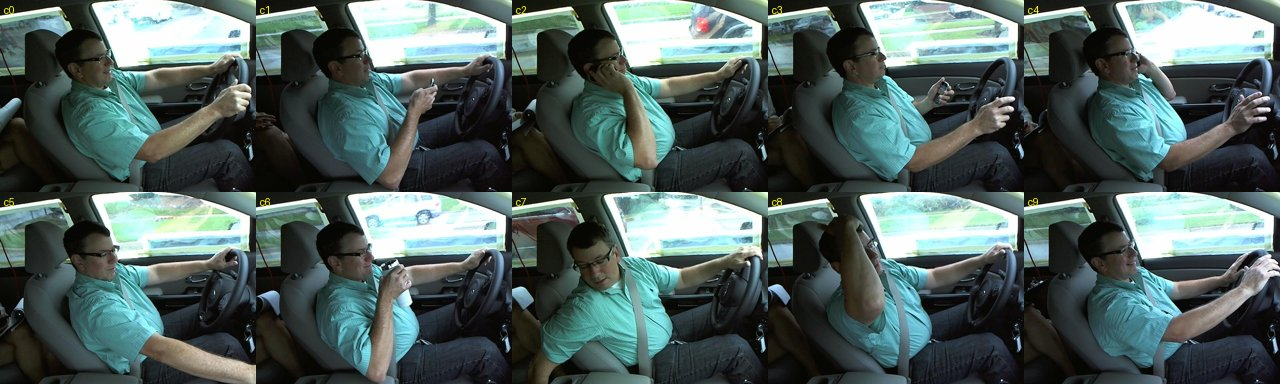
\includegraphics[width=\linewidth]{figs/classes.jpg}\\[-1pt]
{\footnotesize (a) Mười lớp gốc c0--c9 của cùng một tài xế.}\\[4pt]
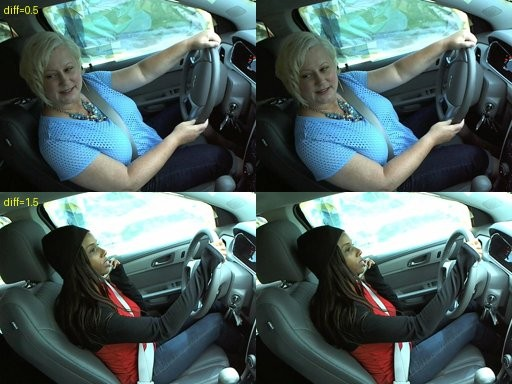
\includegraphics[width=0.62\linewidth]{figs/near_duplicates.jpg}\\[-1pt]
{\footnotesize (b) Hai cặp ảnh gần trùng (sai khác 0,5 và 1,5); chỉ giữ một ảnh mỗi cặp.}
\caption{Dữ liệu State Farm.}
\label{fig:data}
\end{figure}

\subsection{Mô hình và huấn luyện}
\textbf{Kiến trúc.} Bốn mạng phủ một dải quy mô (Bảng~\ref{tab:models}); tất cả dùng trọng số huấn luyện sẵn trên ImageNet, thay lớp phân loại cuối bằng lớp 10 đầu ra và tinh chỉnh toàn bộ.
\begin{itemize}
\item \textbf{MobileNetV3-Small}~\cite{howard2019mobilenetv3}: mô hình mục tiêu cho edge. Dùng tích chập tách theo chiều sâu (một bộ lọc cho mỗi kênh rồi tích chập 1$\times$1 để trộn kênh), giảm mạnh số phép tính so với tích chập thường; khối SE học trọng số cho từng kênh; hàm hard-swish $x\cdot\mathrm{ReLU6}(x+3)/6$ là xấp xỉ rẻ của swish.
\item \textbf{EfficientNet-Lite0}~\cite{tan2019efficientnet,efficientnetlite}: dựa trên EfficientNet-B0, bỏ khối SE và dùng ReLU6, tức các phép toán có miền giá trị bị chặn, thuận lợi cho lượng tử hoá.
\item \textbf{ResNet18 và ResNet50}~\cite{he2016resnet}: mạng dư kinh điển, làm mốc nặng vừa và nặng. ResNet18 dùng khối cơ bản hai lớp 3$\times$3; ResNet50 dùng khối nút cổ chai 1$\times$1--3$\times$3--1$\times$1.
\end{itemize}

\begin{table}[t]
\centering\small
\caption{Quy mô các mô hình (đầu ra 10 lớp, ảnh 224$\times$224). MACs đo bằng bộ đếm phép tính của PyTorch.}
\label{tab:models}
\begin{tabular}{@{}lrrl@{}}
\toprule
Mô hình & Tham số & MACs & Vai trò \\
\midrule
MobileNetV3-Small & 1,53 M & 55 M & ứng viên edge \\
EfficientNet-Lite0 & 3,38 M & 384 M & ứng viên edge \\
ResNet18 & 11,18 M & 1,81 G & mốc nặng vừa \\
ResNet50 & 23,53 M & 4,09 G & mốc nặng \\
\bottomrule
\end{tabular}
\end{table}

\textbf{Huấn luyện.} Mọi mô hình dùng chung một giao thức: 10 epoch, batch 64, AdamW~\cite{loshchilov2019adamw} với learning rate $10^{-3}$ và weight decay $10^{-4}$, lịch học cosine~\cite{loshchilov2017sgdr} giảm về 0 ở epoch cuối, cross-entropy với label smoothing 0,1~\cite{szegedy2016rethinking}, mixed precision trên GPU. Ảnh vào được đưa về 224$\times$224 và chuẩn hoá theo ImageNet. Tăng cường dữ liệu gồm cắt ngẫu nhiên (80--100\% diện tích, tỉ lệ 0,9--1,1), xoay $\pm 8^\circ$, thay đổi độ sáng, tương phản và bão hoà. \emph{Không lật ngang ảnh}, vì lật sẽ biến tay phải thành tay trái và làm sai nhãn của c1--c4. Checkpoint được chọn theo macro-F1 cao nhất trên val; test chỉ được đánh giá một lần với checkpoint đó.

\textbf{Thước đo.} Thước đo chính là macro-F1, trung bình F1 của 10 lớp với trọng số bằng nhau:
\begin{equation}
\mathrm{F1}_c=\frac{2P_cR_c}{P_c+R_c},\qquad \text{macro-F1}=\frac{1}{10}\sum_{c=0}^{9}\mathrm{F1}_c ,
\end{equation}
với $P_c$, $R_c$ là precision và recall của lớp $c$. Mô hình luôn đoán lớp đông nhất ở tập train (c5) cho accuracy 0,117 và macro-F1 0,021 trên test; mọi mô hình phải vượt xa mốc này.

\subsection{Lượng tử hoá INT8 và đo tốc độ}
\label{sec:quant}
\textbf{Lượng tử hoá affine.} Lượng tử hoá ánh xạ một tensor số thực $x$ sang số nguyên 8 bit $q$ bằng một hệ số tỉ lệ $s$ và điểm không $z$~\cite{jacob2018quant}:
\begin{equation}
q=\mathrm{clamp}\!\left(\mathrm{round}\!\left(\tfrac{x}{s}\right)+z,\;q_{\min},q_{\max}\right),\qquad \hat{x}=s\,(q-z).
\end{equation}
Với một khoảng giá trị $[\alpha,\beta]$ cần biểu diễn, $s=(\beta-\alpha)/(q_{\max}-q_{\min})$. Mỗi số chỉ còn 256 mức thay vì số thực 32 bit, nên mô hình nhỏ đi khoảng 4 lần và có thể chạy bằng phép tính số nguyên, nhanh hơn trên phần cứng hỗ trợ. Đổi lại, mỗi giá trị bị làm tròn (sai số tối đa $s/2$) hoặc bị cắt nếu nằm ngoài $[\alpha,\beta]$.

\textbf{Cách làm.} Mô hình PyTorch được xuất sang ONNX (opset 13) rồi lượng tử hoá bằng ONNX Runtime. Cấu hình mặc định là lượng tử hoá \emph{tĩnh} sau huấn luyện: trọng số INT8 với một hệ số cho mỗi kênh đầu ra (per-channel), activation UINT8 với một hệ số cho mỗi tensor, định dạng QDQ (chèn nút Quantize/Dequantize quanh toán tử). Khoảng giá trị của activation được đo trên 200 ảnh huấn luyện (calibration). Chúng tôi so sánh thêm cách chọn khoảng giá trị \emph{minmax} (nhỏ nhất đến lớn nhất), \emph{entropy} (cực tiểu hoá phân kỳ KL) và \emph{percentile} (cắt đuôi phân phối), số ảnh calibration, định dạng QOperator và lượng tử hoá \emph{động} (chỉ trọng số là INT8).

\textbf{Vì sao lượng tử hoá có thể làm giảm độ chính xác.}
(i) Sai số làm tròn ở từng lớp nhỏ nhưng cộng dồn qua hàng chục lớp.
(ii) Một vài giá trị ngoại lai làm khoảng $[\alpha,\beta]$ rộng ra, khiến $s$ lớn và phần lớn giá trị thông thường chỉ còn rất ít mức biểu diễn.
(iii) Trong tích chập theo chiều sâu, mỗi kênh có bộ lọc riêng nên khoảng giá trị khác nhau nhiều giữa các kênh; một hệ số chung cho cả tensor làm mất thông tin ở các kênh nhỏ~\cite{krishnamoorthi2018}.
(iv) Các phép toán như hard-swish và nhánh SE tạo ra phân phối activation khó biểu diễn bằng 8 bit; đây là lý do EfficientNet-Lite bỏ SE và dùng ReLU6~\cite{efficientnetlite}.
Do đó, sau mỗi bước chuyển đổi phải đo lại độ chính xác.

\textbf{Đo tốc độ và cổng khả thi.} Độ trễ đo bằng ONNX Runtime trên CPU Intel Core i5-12400F, 1 luồng, batch 1: 10 lần chạy làm nóng rồi lấy trung vị của 100 lần chạy; FPS $=1000/\text{độ trễ trung vị (ms)}$. Đây là phép xấp xỉ để xếp hạng tương đối, không phải số đo trên chip edge. Một mô hình được coi là \emph{qua cổng khả thi} nếu bản INT8 giảm không quá khoảng 2 điểm macro-F1 so với bản FP32.

% =====================================================================
\section{Thí nghiệm và kết quả}
\textbf{Môi trường.} Huấn luyện chạy trên Google Colab với GPU T4, PyTorch và timm (cho EfficientNet-Lite0). Xuất ONNX, lượng tử hoá và đo tốc độ chạy trên CPU máy cá nhân với ONNX Runtime 1.31. Mã nguồn và nhật ký từng lần chạy nằm trong kho mã của dự án.

\subsection{So sánh mô hình}
Bảng~\ref{tab:main} cho kết quả trên tập test (4 tài xế chưa từng thấy). Mọi mô hình vượt xa mốc đoán lớp đa số (macro-F1 0,021).

\emph{Một lần chia không đủ để xếp hạng.} Bốn mô hình chỉ cách nhau 0,038 về macro-F1 (0,826 đến 0,864). MobileNetV3-Small, mô hình nhỏ nhất, có điểm cao nhất (0,864), còn ResNet50, nặng hơn gần 75 lần về MACs, đạt 0,851. Tuy nhiên cross-validation theo tài xế (mục~\ref{sec:cv}) cho thấy thứ hạng này không bền: MobileNetV3-Small chỉ đạt $0{,}793 \pm 0{,}057$, thấp hơn rõ so với EfficientNet-Lite0 và ResNet18. Điểm 0,864 của nó trên một lần chia nhiều khả năng do 4 tài xế test được chọn tình cờ thuận lợi.

\emph{Val lạc quan hơn test.} Chênh lệch val $-$ test là 0,050 (MobileNetV3-Small), 0,074 (EfficientNet-Lite0), 0,085 (ResNet18) và 0,089 (ResNet50): mô hình càng lớn thì điểm val càng vượt test. Val chỉ có 4 tài xế và được dùng để chọn epoch nên không phản ánh tốt khả năng tổng quát sang tài xế mới.

\emph{Điểm yếu tập trung ở ba lớp.} Bảy lớp còn lại đạt F1 trung bình từ 0,92 đến 0,96, trong khi \cls{c0}, \cls{c8} và \cls{c9} thấp hơn nhiều, nhất là \cls{c9} (0,35 đến 0,57).

\begin{table}[t]
\centering\small
\caption{Kết quả 10 lớp trên một lần chia (test 2.581 ảnh). F1 của ba lớp yếu nhất và trung bình bảy lớp còn lại.}
\label{tab:main}
\setlength{\tabcolsep}{3pt}
\begin{tabular}{@{}lccccccc@{}}
\toprule
Mô hình & Val & Acc & F1 & c0 & c8 & c9 & 7 lớp \\
\midrule
MobileNetV3-S & 0,914 & 0,873 & \textbf{0,864} & 0,66 & 0,77 & 0,57 & 0,95 \\
EfficientNet-Lite0 & 0,918 & 0,856 & 0,844 & 0,83 & 0,66 & 0,45 & 0,93 \\
ResNet18 & 0,911 & 0,835 & 0,826 & 0,77 & 0,69 & 0,37 & 0,92 \\
ResNet50 & 0,940 & 0,872 & 0,851 & 0,71 & 0,74 & 0,35 & 0,96 \\
\midrule
Đoán lớp đa số & -- & 0,117 & 0,021 & -- & -- & -- & -- \\
\bottomrule
\end{tabular}
\end{table}

\subsection{Cross-validation theo tài xế}
\label{sec:cv}
Để đo mức nhiễu của chính phép đánh giá, chúng tôi chia 26 tài xế thành 5 fold; mỗi fold, 5 đến 6 tài xế làm test, 4 tài xế làm val và phần còn lại làm train; mỗi tài xế làm test đúng một lần, và cả ba mô hình dùng cùng các fold. Kết quả ở Bảng~\ref{tab:cv}.

\emph{Xếp hạng khác với một lần chia.} EfficientNet-Lite0 đạt $0{,}863 \pm 0{,}032$, ResNet18 $0{,}855 \pm 0{,}039$ và MobileNetV3-Small chỉ $0{,}793 \pm 0{,}057$. So sánh cặp theo fold (cùng tài xế test): EfficientNet-Lite0 hơn MobileNetV3-Small ở cả 5/5 fold, trung bình $+0{,}070$ (độ lệch chuẩn của hiệu 0,028); ResNet18 hơn MobileNetV3-Small ở 4/5 fold, trung bình $+0{,}061$ (độ lệch chuẩn 0,047, $t=2{,}9$ với 4 bậc tự do, ở mức gần ý nghĩa thống kê, không phải chắc chắn). Giữa EfficientNet-Lite0 và ResNet18 chênh lệch trung bình chỉ $+0{,}009$ (EfficientNet-Lite0 thắng 3/5 fold), tức không phân biệt được. Độ lệch chuẩn theo fold từ 0,03 đến 0,06 cũng lớn hơn khoảng cách giữa các mô hình trên một lần chia, nên điểm một lần chia của MobileNetV3-Small (0,864) cao hơn trung bình CV của nó khoảng 1,2 độ lệch chuẩn.

\emph{Lớp yếu nhất.} \cls{c9} (nói chuyện với hành khách) thấp nhất ở mọi mô hình ($0{,}48$ đến $0{,}60$), theo sau là \cls{c0} (0,62 đến 0,75) và \cls{c8} (0,67 đến 0,79); các lớp còn lại thường đạt 0,85 đến 0,97. MobileNetV3-Small kém hơn cả trên \cls{c0} và \cls{c9}.

\begin{table}[t]
\centering\small
\caption{Cross-validation 5 fold theo tài xế: macro-F1 trên test của từng fold (fold 0 có 6 tài xế test, các fold còn lại 5).}
\label{tab:cv}
\setlength{\tabcolsep}{3pt}
\begin{tabular}{@{}lccccc c@{}}
\toprule
Mô hình & 0 & 1 & 2 & 3 & 4 & TB $\pm$ std \\
\midrule
MobileNetV3-S & 0,733 & 0,853 & 0,822 & 0,826 & 0,732 & $0{,}793 \pm 0{,}057$ \\
EfficientNet-Lite0 & 0,840 & 0,894 & 0,871 & 0,888 & 0,821 & $\mathbf{0{,}863} \pm 0{,}032$ \\
ResNet18 & 0,852 & 0,881 & 0,905 & 0,826 & 0,809 & $0{,}855 \pm 0{,}039$ \\
\midrule
Hiệu E$-$M & +0,108 & +0,042 & +0,049 & +0,062 & +0,089 & $+0{,}070 \pm 0{,}028$ \\
Hiệu E$-$R & $-$0,011 & +0,014 & $-$0,034 & +0,062 & +0,012 & $+0{,}009 \pm 0{,}036$ \\
\bottomrule
\end{tabular}
\end{table}

\subsection{Thử cải thiện}
Trên EfficientNet-Lite0, mỗi lần chỉ đổi một thứ so với cấu hình mặc định (macro-F1 0,844). Augmentation mạnh hơn (cắt rộng hơn, xoay $12^\circ$, đổi màu mạnh, làm mờ, xoá ngẫu nhiên một mảng ảnh) cho 0,858 (+0,014); đưa ảnh vào ở độ phân giải gốc 320$\times$240 thay vì ép vuông 224$\times$224 cho 0,855 (+0,011) nhưng tốn thêm khoảng 1,6 lần MACs (600 M). Cả hai nằm trong phạm vi nhiễu 0,03, nên chúng tôi không kết luận chúng cải thiện thật. Các thay đổi learning rate, weight decay và số epoch thử trên phiên bản 6 nhóm ban đầu cũng không vượt nhiễu.

\subsection{Lượng tử hoá INT8 và tốc độ}
Bảng~\ref{tab:int8} và Hình~\ref{fig:int8} so sánh bản FP32 và INT8 (tĩnh, minmax, per-channel). Bản FP32 xuất qua ONNX cho macro-F1 khớp với PyTorch (sai khác dưới 0,001), xác nhận đường ống xuất mô hình đúng.

\textbf{Ba mô hình giữ được độ chính xác.} EfficientNet-Lite0, ResNet18 và ResNet50 mất không quá 0,008 macro-F1 (với percentile còn không mất), kích thước giảm 3,5 đến 4,0 lần và độ trễ giảm 1,9 đến 3,1 lần. Cả ba qua cổng khả thi, nhưng ResNet50 vẫn rất chậm (46 FPS, so với 215 của EfficientNet-Lite0).

\textbf{MobileNetV3-Small sụp đổ.} Macro-F1 giảm từ 0,864 xuống 0,067. Entropy, percentile, QOperator và lượng tử hoá động đều không cứu được (Mục~\ref{sec:diag}); trên CPU này bản INT8 của nó còn chậm hơn FP32 (463 so với 592 FPS), vì với một mô hình rất nhỏ chi phí của các nút Quantize/Dequantize có thể lớn hơn phần tiết kiệm.

\begin{table}[t]
\centering\small
\caption{FP32 và INT8 trên CPU (ONNX Runtime, 1 luồng, batch 1, test 2.581 ảnh), mô hình 10 lớp.}
\label{tab:int8}
\setlength{\tabcolsep}{3pt}
\begin{tabular}{@{}llrrrc@{}}
\toprule
Mô hình & & MB & ms & FPS & Macro-F1 \\
\midrule
\multirow{2}{*}{MobileNetV3-S} & FP32 & 6,13 & 1,69 & 592 & 0,864 \\
 & INT8 & 1,88 & 2,16 & 463 & \textcolor{red}{0,067} \\
\midrule
\multirow{2}{*}{EfficientNet-Lite0} & FP32 & 13,49 & 8,66 & 115 & 0,844 \\
 & INT8 & 3,81 & 4,65 & 215 & \textbf{0,842} \\
\midrule
\multirow{2}{*}{ResNet18} & FP32 & 44,72 & 29,69 & 34 & 0,826 \\
 & INT8 & 11,30 & 9,63 & 104 & \textbf{0,826} \\
\midrule
\multirow{2}{*}{ResNet50} & FP32 & 94,03 & 66,95 & 15 & 0,851 \\
 & INT8 & 24,04 & 21,76 & 46 & \textbf{0,843} \\
\bottomrule
\end{tabular}
\end{table}

\begin{figure}[t]
\centering
\begin{tikzpicture}
\begin{axis}[
  width=\linewidth, height=5.4cm,
  xlabel={Độ trễ một ảnh trên CPU (ms)},
  ylabel={Macro-F1 trên test},
  xmin=0, xmax=72, ymin=0, ymax=1,
  grid=major, grid style={gray!20},
  legend pos=south east, legend cell align=left,
  nodes near coords, point meta=explicit symbolic,
  every node near coord/.append style={font=\tiny, anchor=west, xshift=2pt},
]
\addplot[only marks, mark=diamond*, mark size=3pt, color=dgray] table[meta=label] {
x y label
1.69 0.864 MobileNetV3-S
8.66 0.844 EffNet-Lite0
29.69 0.826 ResNet18
66.95 0.851 ResNet50
};
\addlegendentry{FP32}
\addplot[only marks, mark=diamond*, mark size=3pt, color=dblue] table[meta=label] {
x y label
4.65 0.842 {}
9.63 0.826 {}
21.76 0.843 {}
};
\addlegendentry{INT8}
\addplot[only marks, mark=diamond*, mark size=3pt, color=dviolet] table[meta=label] {
x y label
2.16 0.067 MobileNetV3-S INT8
};
\addlegendentry{INT8 (sụp)}
\end{axis}
\end{tikzpicture}
\caption{Độ chính xác theo độ trễ, FP32 và INT8. Góc trên bên trái là tốt nhất. EfficientNet-Lite0 INT8 (4,7 ms; 0,842) là mô hình nhanh nhất trong số các mô hình qua được INT8; MobileNetV3-Small INT8 nhanh nhưng sụp về độ chính xác.}
\label{fig:int8}
\end{figure}

\subsection{Chẩn đoán sự sụp đổ của MobileNetV3-Small}
\label{sec:diag}
Chúng tôi tách riêng các nguồn sai số trên MobileNetV3-Small 10 lớp (FP32: 0,864).
\textbf{Không phải lỗi đường ống:} bản FP32 đã qua bước tiền xử lý của bộ lượng tử hoá cho đúng điểm gốc, trọng số trong bản INT8 đúng là per-channel, và tắt toàn bộ tối ưu đồ thị của ONNX Runtime không đổi kết quả.
\textbf{Trọng số lượng tử hoá được:} mô phỏng lượng tử hoá chỉ trọng số, per-channel, cho 0,846; còn per-tensor thì sụp (0,016).
\textbf{Lượng tử hoá activation theo từng loại phép toán} (Bảng~\ref{tab:diag}): lớp phân loại (\texttt{Gemm}), phép cộng và gộp trung bình toàn cục gần như không ảnh hưởng (0,85 đến 0,86), còn \texttt{Conv}, \texttt{Mul} và \texttt{HardSigmoid} làm sập mô hình. Quan trọng là \texttt{Conv} riêng lẻ đã gây sập ngay cả khi \texttt{Mul} và \texttt{HardSigmoid} để FP32, nên nguyên nhân \emph{không} chỉ là hard-swish hay SE như chúng tôi từng giả thuyết, mà là việc lượng tử hoá activation đầu ra của các lớp tích chập.
Cắt khoảng giá trị ở phân vị thấp hơn giúp một phần: phân vị 99,5\% đưa macro-F1 từ 0,067 lên 0,525 (0,567 khi dùng 600 ảnh calibration), nhưng vẫn kém xa FP32. Loại các nhóm lớp nhạy (SE, tích chập theo chiều sâu, lớp đầu, lớp cuối) khỏi lượng tử hoá không cải thiện thêm. Chúng tôi chưa xác định được nguyên nhân sâu hơn (nghi dải giá trị của activation sau BatchNorm); các hướng cần thử tiếp là QAT và biến thể thay hard-swish bằng ReLU6 kèm tinh chỉnh.

\begin{table}[t]
\centering\small
\caption{Lượng tử hoá riêng từng loại phép toán của MobileNetV3-Small (macro-F1 test; FP32 = 0,864).}
\label{tab:diag}
\begin{tabular}{@{}lc@{}}
\toprule
Chỉ lượng tử hoá & Macro-F1 \\
\midrule
\texttt{Gemm} (lớp phân loại) & 0,863 \\
\texttt{Add} & 0,859 \\
\texttt{GlobalAveragePool} & 0,853 \\
\texttt{HardSigmoid} & 0,205 \\
\texttt{Conv} & 0,068 \\
\texttt{Mul} & 0,053 \\
\midrule
Tất cả, minmax (mặc định) & 0,067 \\
Tất cả, percentile 99,5\% & 0,525 \\
Tất cả, percentile 99,5\%, 600 ảnh calibration & 0,567 \\
\bottomrule
\end{tabular}
\end{table}

\subsection{Phân tích lỗi}
Với EfficientNet-Lite0, \cls{c4}, \cls{c7}, \cls{c3}, \cls{c2}, \cls{c1}, \cls{c6} và \cls{c5} đạt F1 từ 0,89 đến 0,98, còn \cls{c8} đạt 0,66 và \cls{c9} chỉ 0,45 (precision 0,66, recall 0,34). Hình~\ref{fig:conf} cho thấy 59\% ảnh \cls{c9} (nói chuyện với hành khách) bị đoán là \cls{c8} (chải tóc, trang điểm), và chỉ 34\% được đoán đúng; ngược lại 16\% ảnh \cls{c8} bị đoán là \cls{c6} (uống nước), và 11\% ảnh \cls{c0} bị đoán là \cls{c9}. Xem trực tiếp các ảnh bị nhầm (Hình~\ref{fig:mis}), phần lớn thuộc về một tài xế (p050) nghiêng đầu sang hành khách, cười và đưa tay lên gần mặt, nên giống hành vi chải tóc; có cả ảnh chỉnh gương mang nhãn \cls{c9}. Lớp c9 vì vậy đa dạng về hình ảnh và có phần nhập nhằng nhãn. Với MobileNetV3-Small, \cls{c9} cũng bị nhầm sang \cls{c8} (40\%) và \cls{c0} bị đoán là \cls{c9} (38\%).

Điểm cũng khác nhiều giữa các tài xế test: với EfficientNet-Lite0, accuracy từ 0,963 (p035) và 0,917 (p042) xuống 0,787 (p081) và 0,779 (p050). Việc tài xế nào rơi vào tập test vì vậy ảnh hưởng đáng kể đến điểm tổng.

\begin{figure}[t]
\centering
\begin{tikzpicture}
\begin{axis}[
  xbar, width=\linewidth, height=3.6cm,
  xmin=0, xmax=75, bar width=7pt,
  xlabel={\% ảnh \cls{c9} (225 ảnh test)},
  symbolic y coords={c1,c0,c9,c8},
  ytick=data, y tick label style={font=\scriptsize\ttfamily},
  nodes near coords, nodes near coords align={horizontal},
  every node near coord/.append style={font=\tiny},
  enlarge y limits=0.2, grid=major, grid style={gray!20},
]
\addplot[fill=dblue!70, draw=none] coordinates {
(0.9,c1) (5.8,c0) (34.2,c9) (59.1,c8)};
\end{axis}
\end{tikzpicture}
\caption{Ảnh có nhãn \cls{c9} được EfficientNet-Lite0 đoán thành lớp nào (dòng \cls{c9} của confusion matrix). Chỉ 34\% được đoán đúng; 59\% bị đoán là \cls{c8}.}
\label{fig:conf}
\end{figure}

\begin{figure}[t]
\centering
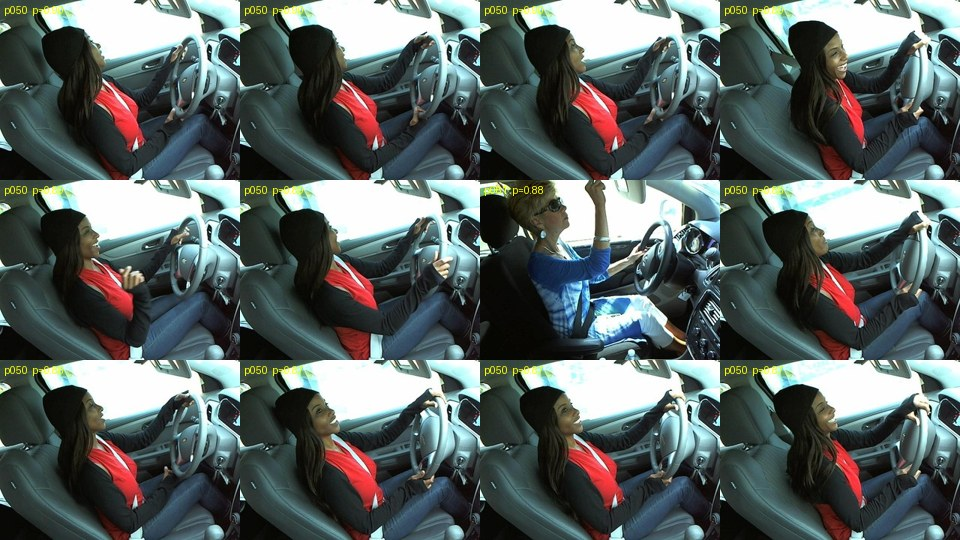
\includegraphics[width=\linewidth]{figs/c9_as_c8.jpg}
\caption{12 ảnh \cls{c9} bị EfficientNet-Lite0 đoán là \cls{c8} với độ tin cậy cao nhất (góc trên: mã tài xế và xác suất). Phần lớn là một tài xế nghiêng đầu sang hành khách và đưa tay gần mặt.}
\label{fig:mis}
\end{figure}

% =====================================================================
\section{Thảo luận}
\textbf{Trả lời câu hỏi nghiên cứu.} Mô hình nặng hơn không chính xác hơn: ResNet50 (4,09 G MACs) không vượt các mô hình nhỏ trên một lần chia, và trong cross-validation ResNet18 (1,81 G) chỉ tương đương EfficientNet-Lite0 (0,38 G). Mô hình nhỏ nhất, MobileNetV3-Small (55 M MACs), lại là mô hình duy nhất bị thiệt rõ rệt, khoảng 0,06 đến 0,07 macro-F1 so với hai mô hình kia, tuy nhiên điều này chỉ lộ ra khi dùng cross-validation (một lần chia cho thứ hạng ngược lại). Ở bước lượng tử hoá, với cùng một phương pháp INT8 sau huấn luyện, EfficientNet-Lite0, ResNet18 và ResNet50 không mất điểm đáng kể, còn MobileNetV3-Small mất gần hết. Như vậy MobileNetV3-Small vừa kém hơn ở FP32 vừa không dùng được sau INT8, nên đánh đổi giữa kích thước và độ chính xác ở đây không phải là một đường thẳng: EfficientNet-Lite0, mô hình trung gian, nằm ở điểm tốt nhất. Số tham số và MACs không đủ để chọn mô hình cho edge; khả năng chịu lượng tử hoá cũng quyết định. Với tiêu chí của bài, EfficientNet-Lite0 INT8 là lựa chọn tốt nhất: macro-F1 0,842, 3,8 MB, 215 FPS trên CPU, nhanh hơn 4,6 lần ResNet50 INT8 ở độ chính xác tương đương.

\textbf{Thu hẹp khoảng cách.} Tăng cường dữ liệu mạnh hơn và ảnh độ phân giải gốc chỉ nâng điểm trong phạm vi nhiễu. Điểm yếu lớn nhất là lớp \cls{c9}, và phân tích lỗi cho thấy nguyên nhân chủ yếu nằm ở dữ liệu (ảnh đa dạng, nhập nhằng với \cls{c8}, tập trung ở vài tài xế) hơn là ở kiến trúc, vì mọi mô hình đều yếu ở lớp này.

\textbf{Hạn chế.} (i) Mỗi tập val và test chỉ có 4 tài xế; cross-validation cho độ lệch chuẩn 0,03 đến 0,06 theo fold, và chỉ có 5 fold nên kiểm định cặp có rất ít bậc tự do. Cross-validation chạy cho ba mô hình, không gồm ResNet50 và các cấu hình thử cải thiện, nên các so sánh đó vẫn chỉ dựa trên một lần chia. (ii) Mỗi cấu hình chỉ chạy một seed. (iii) Tốc độ đo trên CPU máy tính, chỉ để so sánh tương đối; FPS và khả năng hỗ trợ toán tử trên chip edge thật cần đo riêng. (iv) Nguyên nhân sâu xa của sự sụp đổ INT8 ở MobileNetV3-Small chưa được xác định và chưa thử QAT. (v) Chỉ dùng một bộ dữ liệu, một góc camera.

% =====================================================================
\section{Kết luận}
Bài này so sánh bốn mạng tích chập cho bài toán nhận diện tài xế mất tập trung trên thiết bị edge, với 10 lớp hành vi, chia theo tài xế và loại bỏ ảnh gần trùng. Trên một lần chia, bốn mô hình có độ chính xác gần ngang nhau (macro-F1 0,83 đến 0,86), nhưng cross-validation 5 fold theo tài xế cho thấy MobileNetV3-Small ($0{,}793 \pm 0{,}057$) kém hơn rõ so với EfficientNet-Lite0 ($0{,}863 \pm 0{,}032$) và ResNet18 ($0{,}855 \pm 0{,}039$), hai mô hình này không phân biệt được; mô hình nặng không chính xác hơn. Về lượng tử hoá INT8, EfficientNet-Lite0 giữ nguyên độ chính xác, nhỏ hơn 3,5 lần và nhanh hơn 1,9 lần, trong khi MobileNetV3-Small không chịu được INT8 sau huấn luyện. EfficientNet-Lite0 vì vậy là lựa chọn tốt nhất cho edge. Bài học phương pháp: xếp hạng từ một lần chia theo tài xế có thể bị đảo ngược. Chẩn đoán cho thấy nguyên nhân là lượng tử hoá activation của các lớp tích chập chứ không chỉ hard-swish hay SE. Hướng phát triển gồm: cross-validation cho ResNet50 và nhiều seed, QAT hoặc biến thể ReLU6 cho MobileNetV3-Small, đo trên chip edge thật, chưng cất tri thức từ mô hình lớn sang mô hình nhỏ, và xem lại nhãn của lớp \cls{c9}.

% =====================================================================
\begin{thebibliography}{99}\small
\bibitem{statefarm} State Farm, ``State Farm Distracted Driver Detection,'' Kaggle competition, 2016. \url{https://www.kaggle.com/c/state-farm-distracted-driver-detection}
\bibitem{he2016resnet} K. He, X. Zhang, S. Ren, J. Sun, ``Deep residual learning for image recognition,'' in \emph{CVPR}, 2016.
\bibitem{howard2019mobilenetv3} A. Howard \emph{et al.}, ``Searching for MobileNetV3,'' in \emph{ICCV}, 2019.
\bibitem{hu2018senet} J. Hu, L. Shen, G. Sun, ``Squeeze-and-excitation networks,'' in \emph{CVPR}, 2018.
\bibitem{tan2019efficientnet} M. Tan, Q. V. Le, ``EfficientNet: Rethinking model scaling for convolutional neural networks,'' in \emph{ICML}, 2019.
\bibitem{efficientnetlite} R. Liu, ``Higher accuracy on vision models with EfficientNet-Lite,'' TensorFlow Blog, 2020.
\bibitem{jacob2018quant} B. Jacob \emph{et al.}, ``Quantization and training of neural networks for efficient integer-arithmetic-only inference,'' in \emph{CVPR}, 2018.
\bibitem{krishnamoorthi2018} R. Krishnamoorthi, ``Quantizing deep convolutional networks for efficient inference: A whitepaper,'' arXiv:1806.08342, 2018.
\bibitem{nagel2021white} M. Nagel \emph{et al.}, ``A white paper on neural network quantization,'' arXiv:2106.08295, 2021.
\bibitem{loshchilov2019adamw} I. Loshchilov, F. Hutter, ``Decoupled weight decay regularization,'' in \emph{ICLR}, 2019.
\bibitem{loshchilov2017sgdr} I. Loshchilov, F. Hutter, ``SGDR: Stochastic gradient descent with warm restarts,'' in \emph{ICLR}, 2017.
\bibitem{szegedy2016rethinking} C. Szegedy \emph{et al.}, ``Rethinking the Inception architecture for computer vision,'' in \emph{CVPR}, 2016.
\end{thebibliography}

\end{document}
